\documentclass[noauthor,nooutcomes,12pt,hints,handout]{ximera}

\graphicspath{  
{./}
{./whoAreYou/}
{./drawingWithTheTurtle/}
{./bisectionMethod/}
{./circles/}
{./anglesAndRightTriangles/}
{./lawOfSines/}
{./lawOfCosines/}
{./plotter/}
{./staircases/}
{./pitch/}
{./qualityControl/}
{./symmetry/}
{./nGonBlock/}
}


%% page layout
\usepackage[cm,headings]{fullpage}
\raggedright
\setlength\headheight{13.6pt}


%% fonts
\usepackage{euler}

\usepackage{FiraMono}
\renewcommand\familydefault{\ttdefault} 
\usepackage[defaultmathsizes]{mathastext}
\usepackage[htt]{hyphenat}

\usepackage[T1]{fontenc}
\usepackage[scaled=1]{FiraSans}

%\usepackage{wedn}
\usepackage{pbsi} %% Answer font


\usepackage{cancel} %% strike through in pitch/pitch.tex


%% \usepackage{ulem} %% 
%% \renewcommand{\ULthickness}{2pt}% changes underline thickness

\tikzset{>=stealth}

\usepackage{adjustbox}

\setcounter{titlenumber}{-1}

%% journal style
\makeatletter
\newcommand\journalstyle{%
  \def\activitystyle{activity-chapter}
  \def\maketitle{%
    \addtocounter{titlenumber}{1}%
                {\flushleft\small\sffamily\bfseries\@pretitle\par\vspace{-1.5em}}%
                {\flushleft\LARGE\sffamily\bfseries\thetitlenumber\hspace{1em}\@title \par }%
                {\vskip .6em\noindent\textit\theabstract\setcounter{question}{0}\setcounter{sectiontitlenumber}{0}}%
                    \par\vspace{2em}
                    \phantomsection\addcontentsline{toc}{section}{\thetitlenumber\hspace{1em}\textbf{\@title}}%
                     }}
\makeatother



%% thm like environments
\let\question\relax
\let\endquestion\relax

\newtheoremstyle{QuestionStyle}{\topsep}{\topsep}%%% space between body and thm
		{}                      %%% Thm body font
		{}                              %%% Indent amount (empty = no indent)
		{\bfseries}            %%% Thm head font
		{)}                              %%% Punctuation after thm head
		{ }                           %%% Space after thm head
		{\thmnumber{#2}\thmnote{ \bfseries(#3)}}%%% Thm head spec
\theoremstyle{QuestionStyle}
\newtheorem{question}{}



\let\freeResponse\relax
\let\endfreeResponse\relax

%% \newtheoremstyle{ResponseStyle}{\topsep}{\topsep}%%% space between body and thm
%% 		{\wedn\bfseries}                      %%% Thm body font
%% 		{}                              %%% Indent amount (empty = no indent)
%% 		{\wedn\bfseries}            %%% Thm head font
%% 		{}                              %%% Punctuation after thm head
%% 		{3ex}                           %%% Space after thm head
%% 		{\underline{\underline{\thmname{#1}}}}%%% Thm head spec
%% \theoremstyle{ResponseStyle}

\usepackage[tikz]{mdframed}
\mdfdefinestyle{ResponseStyle}{leftmargin=1cm,linecolor=black,roundcorner=5pt,
, font=\bsifamily,}%font=\wedn\bfseries\upshape,}


\ifhandout
\NewEnviron{freeResponse}{}
\else
%\newtheorem{freeResponse}{Response:}
\newenvironment{freeResponse}{\begin{mdframed}[style=ResponseStyle]}{\end{mdframed}}
\fi



%% attempting to automate outcomes.

%% \newwrite\outcomefile
%%   \immediate\openout\outcomefile=\jobname.oc
%% \renewcommand{\outcome}[1]{\edef\theoutcomes{\theoutcomes #1~}%
%% \immediate\write\outcomefile{\unexpanded{\outcome}{#1}}}

%% \newcommand{\outcomelist}{\begin{itemize}\theoutcomes\end{itemize}}

%% \NewEnviron{listOutcomes}{\small\sffamily
%% After answering the following questions, students should be able to:
%% \begin{itemize}
%% \BODY
%% \end{itemize}
%% }
\usepackage[tikz]{mdframed}
\mdfdefinestyle{OutcomeStyle}{leftmargin=2cm,rightmargin=2cm,linecolor=black,roundcorner=5pt,
, font=\small\sffamily,}%font=\wedn\bfseries\upshape,}
\newenvironment{listOutcomes}{\begin{mdframed}[style=OutcomeStyle]After answering the following questions, students should be able to:\begin{itemize}}{\end{itemize}\end{mdframed}}



%% my commands

\newcommand{\snap}{{\bfseries\itshape\textsf{Snap!}}}
\newcommand{\flavor}{\link[\snap]{https://snap.berkeley.edu/}}
\newcommand{\mooculus}{\textsf{\textbf{MOOC}\textnormal{\textsf{ULUS}}}}


\usepackage{tkz-euclide}
\tikzstyle geometryDiagrams=[rounded corners=.5pt,ultra thick,color=black]
\colorlet{penColor}{black} % Color of a curve in a plot



\ifhandout\newcommand{\mynewpage}{\newpage}\else\newcommand{\mynewpage}{}\fi


\author{Bart Snapp}

\title{Types of symmetry}

\begin{document}
\begin{abstract}
  We organize our symmetries by what they do.
\end{abstract}
\maketitle

\begin{listOutcomes}
\item Organize symmetries of the regular $n$-gon into types.
\item View the infinite number of translational symmetries of a frieze
  pattern as a single TYPE of symmetry.
\item Use \snap\ to experiment with the symmetries of different frieze
  patterns.
\item Identify frieze patterns with various combinations of
  symmetries.
\item Explain why there are certain combinations of symmetries that no
  frieze pattern has.
\end{listOutcomes}

Frieze patterns have really different symmetries than regular
$n$-gons.
\begin{itemize}
  \item A \textbf{regular $\boldsymbol n$-gon} ALWAYS has a FINITE
    number of symmetries, namely $2n$.
  \item A \textbf{frieze pattern} ALWAYS has an INFINITE number of symmetries,
    since we can translate (to the left or right) by
    \begin{align*}
      1\ &\text{minimal cell}\\
      2\ &\text{minimal cells}\\
      &\vdots \\
      n\ &\text{minimal cells}\\
      &\vdots
    \end{align*}
\end{itemize}
Here's an idea: Let's ORGANIZE the symmetries by \textbf{what they
  do}. For example, a regular $n$-gon has TWO TYPES of symmetries,
\begin{itemize}
\item ROTATIONS: $e,r,r^2,\dots,r^n$ and
\item FLIPS: $f,rf,r^2f,\dots,r^nf$.
\end{itemize}

Frieze patterns now ALWAYS have AT LEAST one type of symmetry:
Translations.


\textbf{Let's discover more types of symmetry that
  frieze patterns can have}.

As a gesture of friendship, I give you the FRIEZE-EXPLORER-BLOCK:
\begin{center}
  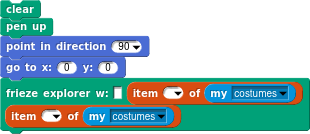
\includegraphics{friezeExplorerSCRIPT.png}
\end{center}




\mynewpage



\begin{question}
  There are other symmetries that frieze patterns can have. Here are
  three more:
  \begin{enumerate}
  \item glide-reflections
  \item vertical-reflections
  \item $180^\circ$ rotations
  \end{enumerate}
  Use the INTERNET to EXPLAIN what each of these symmetries are as you
  would like them explained to you. You should use words, pictures,
  and so on as needed/helpful in your explanation.
  \begin{freeResponse}
    \begin{enumerate}
    \item A glide-reflection is a combination of a translation and a
      vertical-reflection.
    \item A vertical-reflection is a reflection across a horizontal
      line, presumably a line through the center of the frieze
      pattern.
    \item An $180^\circ$ rotation is spinning the frieze pattern
      $180^\circ$. To have symmetry through a $180^\circ$ rotation
      means that the frieze pattern looks the same right-side-up as it
      does up-side-down.
    \end{enumerate}
  \end{freeResponse}
\end{question}

\mynewpage

\begin{question}
  Every frieze pattern has symmetry though translations.
  \begin{enumerate}
    \item DISPLAY a frieze pattern that has symmetry through
      translations and glide-reflections, but no others.
    \item Can you find a frieze pattern that has symmetry through
    glide-reflections but not though vertical-reflections? If YES, show
    me such a frieze pattern. If NO, explain why not.
  \end{enumerate}
  \begin{freeResponse}
    \begin{enumerate}
      \item Here is a frieze pattern with symmetries through
        translations and glide-reflections, but no others.
        \begin{center}
          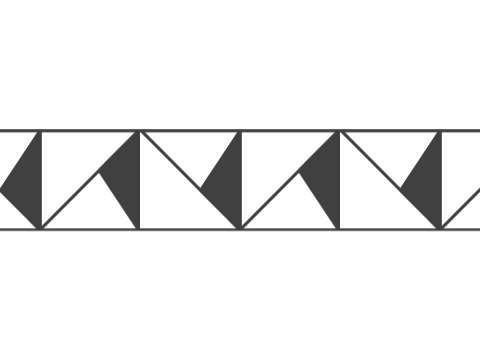
\includegraphics[width=.6\textwidth]{ansGR.png}
        \end{center}
      \item NO, every frieze with symmetry through translations and
        vertical-reflections will automatically have symmetry through
        glide-reflections.
    \end{enumerate}
  \end{freeResponse}
\end{question}
\mynewpage

\begin{question}
  In a similar theme to the last problem\dots 
  \begin{enumerate}
    \item Can you find a frieze pattern that has symmetry through
      $180^\circ$ rotations but not though glide-reflections or
      vertical-reflections? If YES, show me such a frieze pattern. If
      NO, explain why not.
      
    \item Can you find a frieze pattern that has symmetry through
      vertical-reflections and $180^\circ$ rotations but not though
      glide-reflections? If YES, show me such a frieze pattern. If NO,
      explain why not.

    \item Can you find a frieze pattern that has symmetry through
      glide-reflections and $180^\circ$ rotations but not though
      vertical-reflections? If YES, show me such a frieze pattern. If
      NO, explain why not.
  \end{enumerate}
  \begin{freeResponse}
    \begin{enumerate}
    \item Here is a frieze pattern with symmetries through
      translations and $180^\circ$ rotations, but no others.
      \begin{center}
        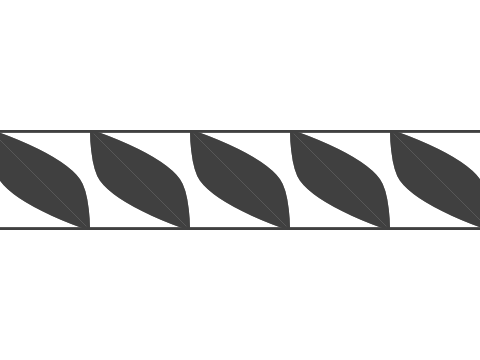
\includegraphics[width=.6\textwidth]{ansR.png}
      \end{center}
    \item NO again, every frieze with vertical reflections will also
      have symmetry through translations and vertical-reflections,
      which means the frieze pattern will ALSO have symmetry through
      glide-reflections.
    \item Here is a frieze pattern with symmetries through
      translations, glide-reflections, and $180^\circ$ rotations but
      not vertical-reflections.
        \begin{center}
          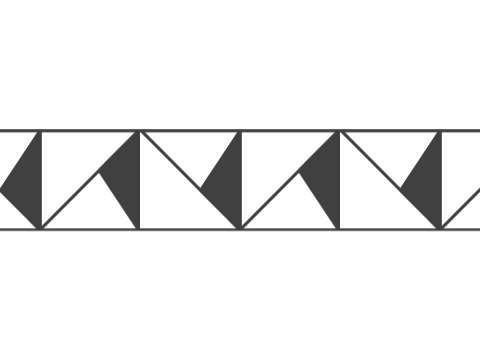
\includegraphics[width=.6\textwidth]{ansGR.png}
        \end{center}
        Note, this one does seem to have symmetry through HORIZONTAL
        reflections.
    \end{enumerate}
  \end{freeResponse}
\end{question}




\end{document}
